\documentclass[TechnicalNoteMeteo.tex]{subfiles}

\begin{document}

\subsection{Materials and Method}

\subsubsection{Study Area}

The method was tested using data from land-based Canadian weather stations located in and around the Monteregie Est region, which is located in southern Quebec, Canada. This region covers a total area of \SI{9032}{km^2}, from the St. Lawrence River at its northern limit to the border of the United States (states of New York and Vermont) at its southern limit (see Figure X). It is characterized by strongly variable topography and land cover conditions. The climate of this region is characterized by significant seasonal differences in temperature, resulting in warm summers and cold winters. Total precipitation, as rain or snow, are distributed rather evenly throughout the year.

\subsubsection{Weather Dataset}

Among all the weather stations for which data were available in and around the study area in the Canadian Daily Climate Database (CDCD), a total of 32 was selected based on the availability and continuity of the measured weather data between 1980 and 2014. \Cref{tab:selectedStations} presents the list of these selected stations with their corresponding climate~ID, location coordinates (latitude and longitude), altitude, time periods for which data were available, mean annual cumulative precipitation, and mean annual air temperature. Most of the information presented in \cref{tab:selectedStations} are generated automatically when loading data into the gap-filling routine and saved in a file named `weather\_datasets\_summary.log' within the previously defined output folder. The geographical disposition of the weather stations is also presented in the map of \cref{fig:Thiessen_meteo}.

The data were downloaded and formatted to the format described in section X using the software WHAT \citep{gosselin_user_2015}. In addition to offering a set of tools to assist in the interpretation of water level time series, WHAT also provides a graphical interface to the online CDCD that allows to search for stations interactively using location coordinates, download the available data for the selected weather stations, and automatically organize the data in a more convenient format. As mentioned previously, it also included an interface to easily use the gap-filling algorithm presented in this paper.

\begin{table}[!ht]
    \centering
    \caption{List of selected weather stations in the study area and related information about missing data for the 1980-2014 period}
    \rowcolors{6}{gray!10}{}
    \resizebox{0.65\linewidth}{!}{
    \begin{tabular}{            
        S[table-format = 2]
        l
        *2S[table-format = 2.2]
        S[table-format = 3.1]
        *4S[table-format = 2.1]
        S[table-format = 2.1]
        S[table-format = -1.1]
        S[table-format = 1.1]
        S[table-format = 4.1]
    	}
    	\toprule
    	\multicolumn{5}{c}{} & \multicolumn{4}{c}{\% of days with missing data} & \multicolumn{4}{c}{Yearly Averages}\\
    	\cmidrule(lr){6-9}
    	\cmidrule(lr){10-13}
    	{\#} & {Station} & {Lat.} & {Lon.} & {Alt.} & {T\textsubscript{max}} & {T\textsubscript{min}} & {T\textsubscript{mean}} & {P\textsubscript{tot}} & {T\textsubscript{max}} & {T\textsubscript{min}} & {T\textsubscript{mean}} & {P\textsubscript{tot}} \\
    	& {name} & {\SIUnitSymbolDegree N} & {\SIUnitSymbolDegree W} & {m} & {\%} & {\%} & {\%} & {\%} & {\SIUnitSymbolCelsius} & {\SIUnitSymbolCelsius} & {\SIUnitSymbolCelsius} & {mm} \\
    	\midrule
        1 & Auteuil & 45.65 & 73.73 & 53.0 & 20.8 & 19.1 & 22.8 & 18.4 & 11.3 & 1.4 & 6.4 & 989.7 \\
        2 & Bonsecours & 45.40 & 72.27 & 297.2 & 4.7 & 5.1 & 6.3 & 3.2 & 10.0 & -0.8 & 4.6 & 1226.2 \\
        3 & Brome & 45.18 & 72.57 &  205.7 & 2.6 & 2.3 & 3.0 & 2.3 & 11.0 & -0.4 & 5.3 & 1296.7 \\
        4 & Bromptonville & 45.48 &  71.95 &  130.0 & 3.9 & 4.2 & 6.0 & 1.8 & 11.1 & -0.1 & 5.5 & 1137.9 \\
        5 & Danville & 45.82 & 71.98 & 190.0 & 30.8 & 31.1 & 33.1& 30.2 & 10.6 & 0.4 & 5.5 & 1074.5 \\
        6 & Drummondville & 45.88 & 72.48 & 82.3 & 2.5 & 2.4 & 3.4 & 1.8 & 11.0 & 1.5 & 6.2 & 1122.1 \\
        7 & Farnham & 45.30 & 72.90 & 68.0 & 5.2 & 4.7 & 6.1 & 3.7 \\
        8 & Fleury & 45.80 & 73.00 & 30.5 & 1.1 & 1.2 & 1.6 & 1.1 \\
        9 & Georgeville & 45.13 & 72.23 & 266.7 & 26.5 & 26.2 & 27.6 & 5.7 \\
        10 & Granby & 45.38 & 72.72 & 175.0 & 1.3 & 1.3 & 2.1 & 0.5 \\
        11 & Hemmingford & 45.07 & 73.72 & 61.0 & 6.0 & 6.0 & 6.8 & 4.6 \\
        12 & Iberville & 45.33 & 73.25 & 30.5 & 7.3 & 7.5 & 9.7 & 4.2 \\
        13 & Magog & 45.27 & 72.12 & 274.0 & 4.2 & 4.2 & 5.3 & 4.6 \\
        14 & Marieville & 45.40 & 73.13 & 38.0 & 10.2 & 10.4 & 11.2 & 9.8 \\
        15 & Nicolet & 46.20 & 72.62 & 30.4 & 4.1 & 4.2 & 5.2 & 3.6 \\
        16 & Philipsburg & 45.03 & 73.08 & 53.3 & 4.9 & 5.1 & 6.9 & 3.2 \\
        17 & Pierreville & 46.08 & 72.83 & 15.2 & 6.3 & 5.4 & 6.9 & 4.9 \\
        18 & Richmond  & 45.63 & 72.13 & 123.1 & 3.3 & 3.3 & 3.8 & 4.0 \\
        19 & Riviere des Prairies & 45.70 & 73.50 & 9.0 & 2.4 & 4.0 & 4.8 & 1.4 \\
        20 & Sabrevois & 45.22 & 73.20 & 38.1 & 25.5 & 26.0 & 27.1 & 5.2 \\
        21 & Sorel & 46.03 & 73.12 & 14.6 & 5.7 & 5.9 & 6.2 & 4.5 \\
        22 & St. Amable & 45.67 & 73.30 & 41.1 & 8.6 & 10.4 & 11.8 & 7.7 \\
        23 & St. Bernard & 45.08 & 73.38 & 49.3 & 9.6 & 9.7 & 10.5 & 9.0 \\
        24 & St. Guillaume & 45.88 & 72.77 & 43.9 & 4.3 & 4.6 & 5.7 & 3.0 \\
        25 & St.Hyacinthe 2 & 45.57 & 72.92 & 33.0 & 6.7 & 6.9 & 7.5 & 6.6 \\
        26 & St. Jacques & 45.95 & 73.58 & 69.0 & 11.7 & 11.9 & 14.0 & 10.8 \\
        27 & St. Janvier & 45.73 & 73.88 & 61.0 & 40.5 & 40.7 & 41.6 & 21.9 \\
        28 & St. Nazaire & 45.73 & 72.62 & 68.6 & 3.8 & 3.8 & 5.4 & 2.7 \\
        29 & Ste. Madeleine & 45.62 & 73.13 & 30.0 & 5.8 & 6.4 & 7.0 & 5.1 \\
        30 & Ste. Martine & 45.22 & 73.85 & 38.1 & 6.9 & 6.6 & 7.8 & 6.4 \\
        31 & Sutton & 45.07 & 72.68 & 243.8 & 0.4 & 0.6 & 0.7 & 0.5 \\
        32 & Vercheres & 45.77 & 73.37 & 21.0 & 3.5 & 3.5 & 4.7 & 2.2 \\
        \bottomrule
    \end{tabular}
    }
    \label{tab:selectedStations}
\end{table}

Total annual precipitation for all of these stations, the mean annual precipitation is \SI{1100}{mm/y}. The highest total precipitation are observed at the Brome station ($\sim$\SI{1280}{mm/y}), while the lowest at the Sorel station ($\sim$\SI{960}{mm/year}). Mean annual air temperature in the study area is \SI{5.9}{\celsius}, ranging from \SIrange{4.3}{6.7}{\celsius} while average monthly temperatures fluctuate between \SIrange{-12}{21}{\celsius}. The minimum monthly temperatures are observed in January \SIrange{-17.1}{-13.6}{\celsius}) while the maximum monthly temperatures are observed in July (\SIrange{24}{26.7}{\celsius}).
The highest temperatures are observed at the Philipsburg et Saint-Bernard stations and the lowest at Bonsecours station.

%Dans la région d‘étude, la tendance générale indique que les précipitations annuelles totales diminuent du sud-sud-est vers le nord-nord-ouest et que les températures annuelles moyennes diminuent du sud-ouest vers le nord-est. Outre l‘influence de la latitude, la température de la région est également influencée par la présence des Appalaches au sud-est et du fleuve Saint-Laurent au nord-ouest. Les figures 1.3 et 1.4 illustrent respectivement les variations spatiales des précipitations totales annuelles et de la température moyenne annuelle pour la période de 1970-2000. Les valeurs présentées sur ces figures ont été interpolées par krigeage ordinaire sur une grille de 250 x 250 m, à partir des valeurs rapportées pour les 16 stations actives mentionnées ci-haut.

\begin{figure}
\centering
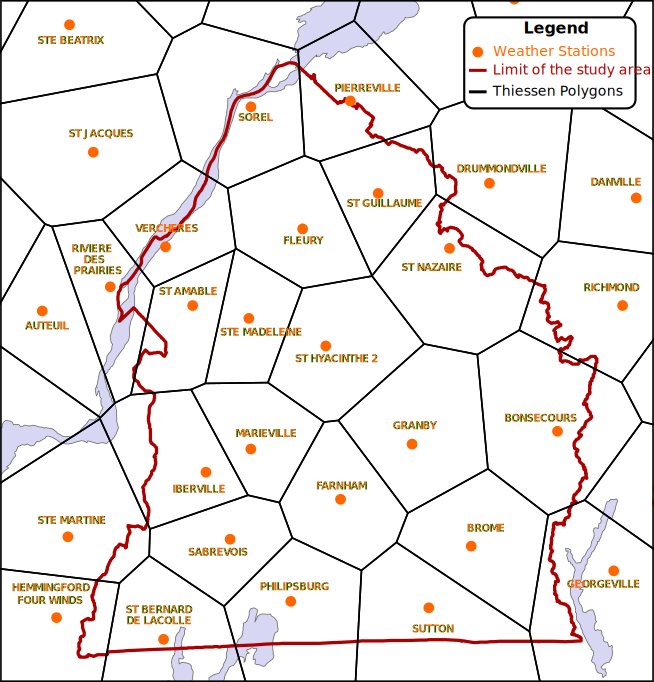
\includegraphics[width=0.75\textwidth]{img/Thiessen_meteo}
\caption[Locations of the weather stations in the Monteregie Est area.]{Locations of the weather stations in the Monteregie Est area.}
\label{fig:Thiessen_meteo}
\end{figure}

\subsubsection{Gap-Filling the Data}
The algorithm described in \cref{sec:Theory} of this paper was used to estimate the missing weather data and fill the gaps in the weather dataset of the station located within the study area. Stations bordering the limits but outside the study area were used to fill the data of the stations within the area, but their data were not filled. Data from these stations were use only to improve the spatial distribution of the neighboring stations for the weather station in the study area located near the limits.

The default value for the method parameters were kept in the algorithm. That is, the maximum number of neighboring station was set to 4, the horizontal and vertical distance thresholds were kept at 100 and 350 values respectively. The data were filled using the OLR and LRM method to see if it makes any real difference. Also, during the entire process, the option for the cross-validation was activated.

The accuracy of the method was also assessed with different value imposed on the maximum number of neighboring stations to see the impact on the accuracy of the method.

\end{document}

%The Canadian Daily Climate Database (CDCD), owned by the Government of Canada, contains daily data for air temperature and precipitation dating back to 1840 to the present for about 8450 stations distributed across Canada. Data can be downloaded manually on the Government of Canada website (\url{www.climate.weather.gc.ca}) for each year individually and saved in a csv file. This process involves a lot of repetitive manipulations and is a time consuming task. Moreover, the re-organization of the individual data files, saved for each year separately, in a more convenient format can also represent a tedious task when done manually. Alternatively, it is possible to order a DVD containing the entire database for a small fee. This option has the disadvantage of only providing an image in time as data cannot be updated.  

%This region has been the subject of an extensive characterization project within the `Programme d'acquisition de connaissances sur les eaux souterraines du Québec' (PACES) whose main objective was to prepare a realistic and concrete picture of the groundwater resources for the region \citep{carrier_portrait_2013}.